\setcounter{section}{3}
\setcounter{subsection}{3}
\setcounter{subsubsection}{4}

\subsubsection{Mixed Scheduling}
Theoretically, the background tasks should fill in the gaps at $600 < t < 700$ and $1100 < t < 1300$ in the schedule.
\begin{figure}[H]
    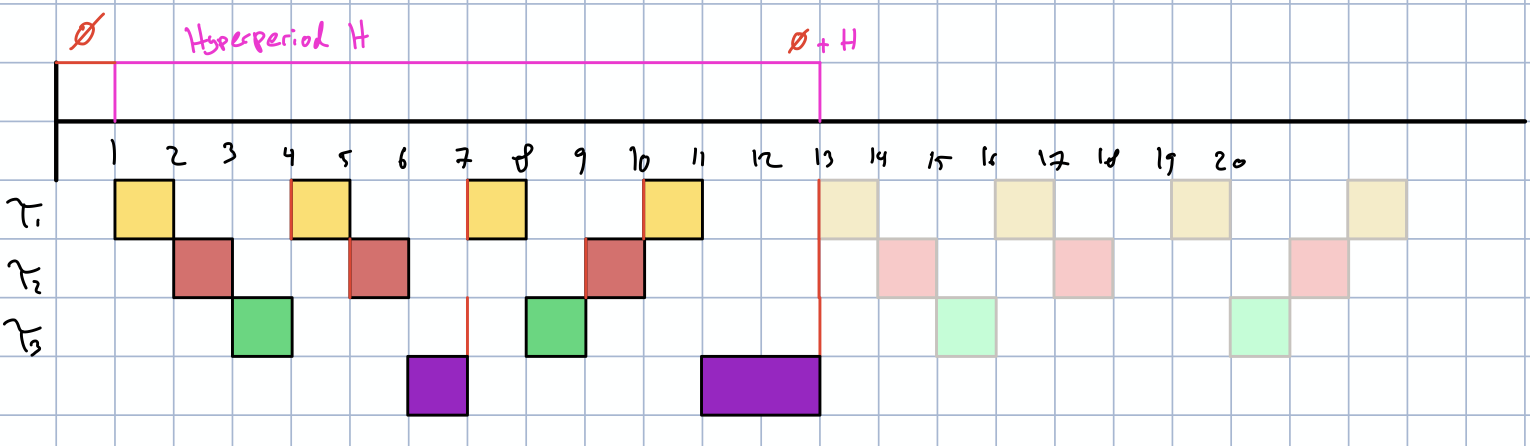
\includegraphics[width=\linewidth]{background-tasks-schedule}
\end{figure}

The command output:
\begin{figure}[H]
    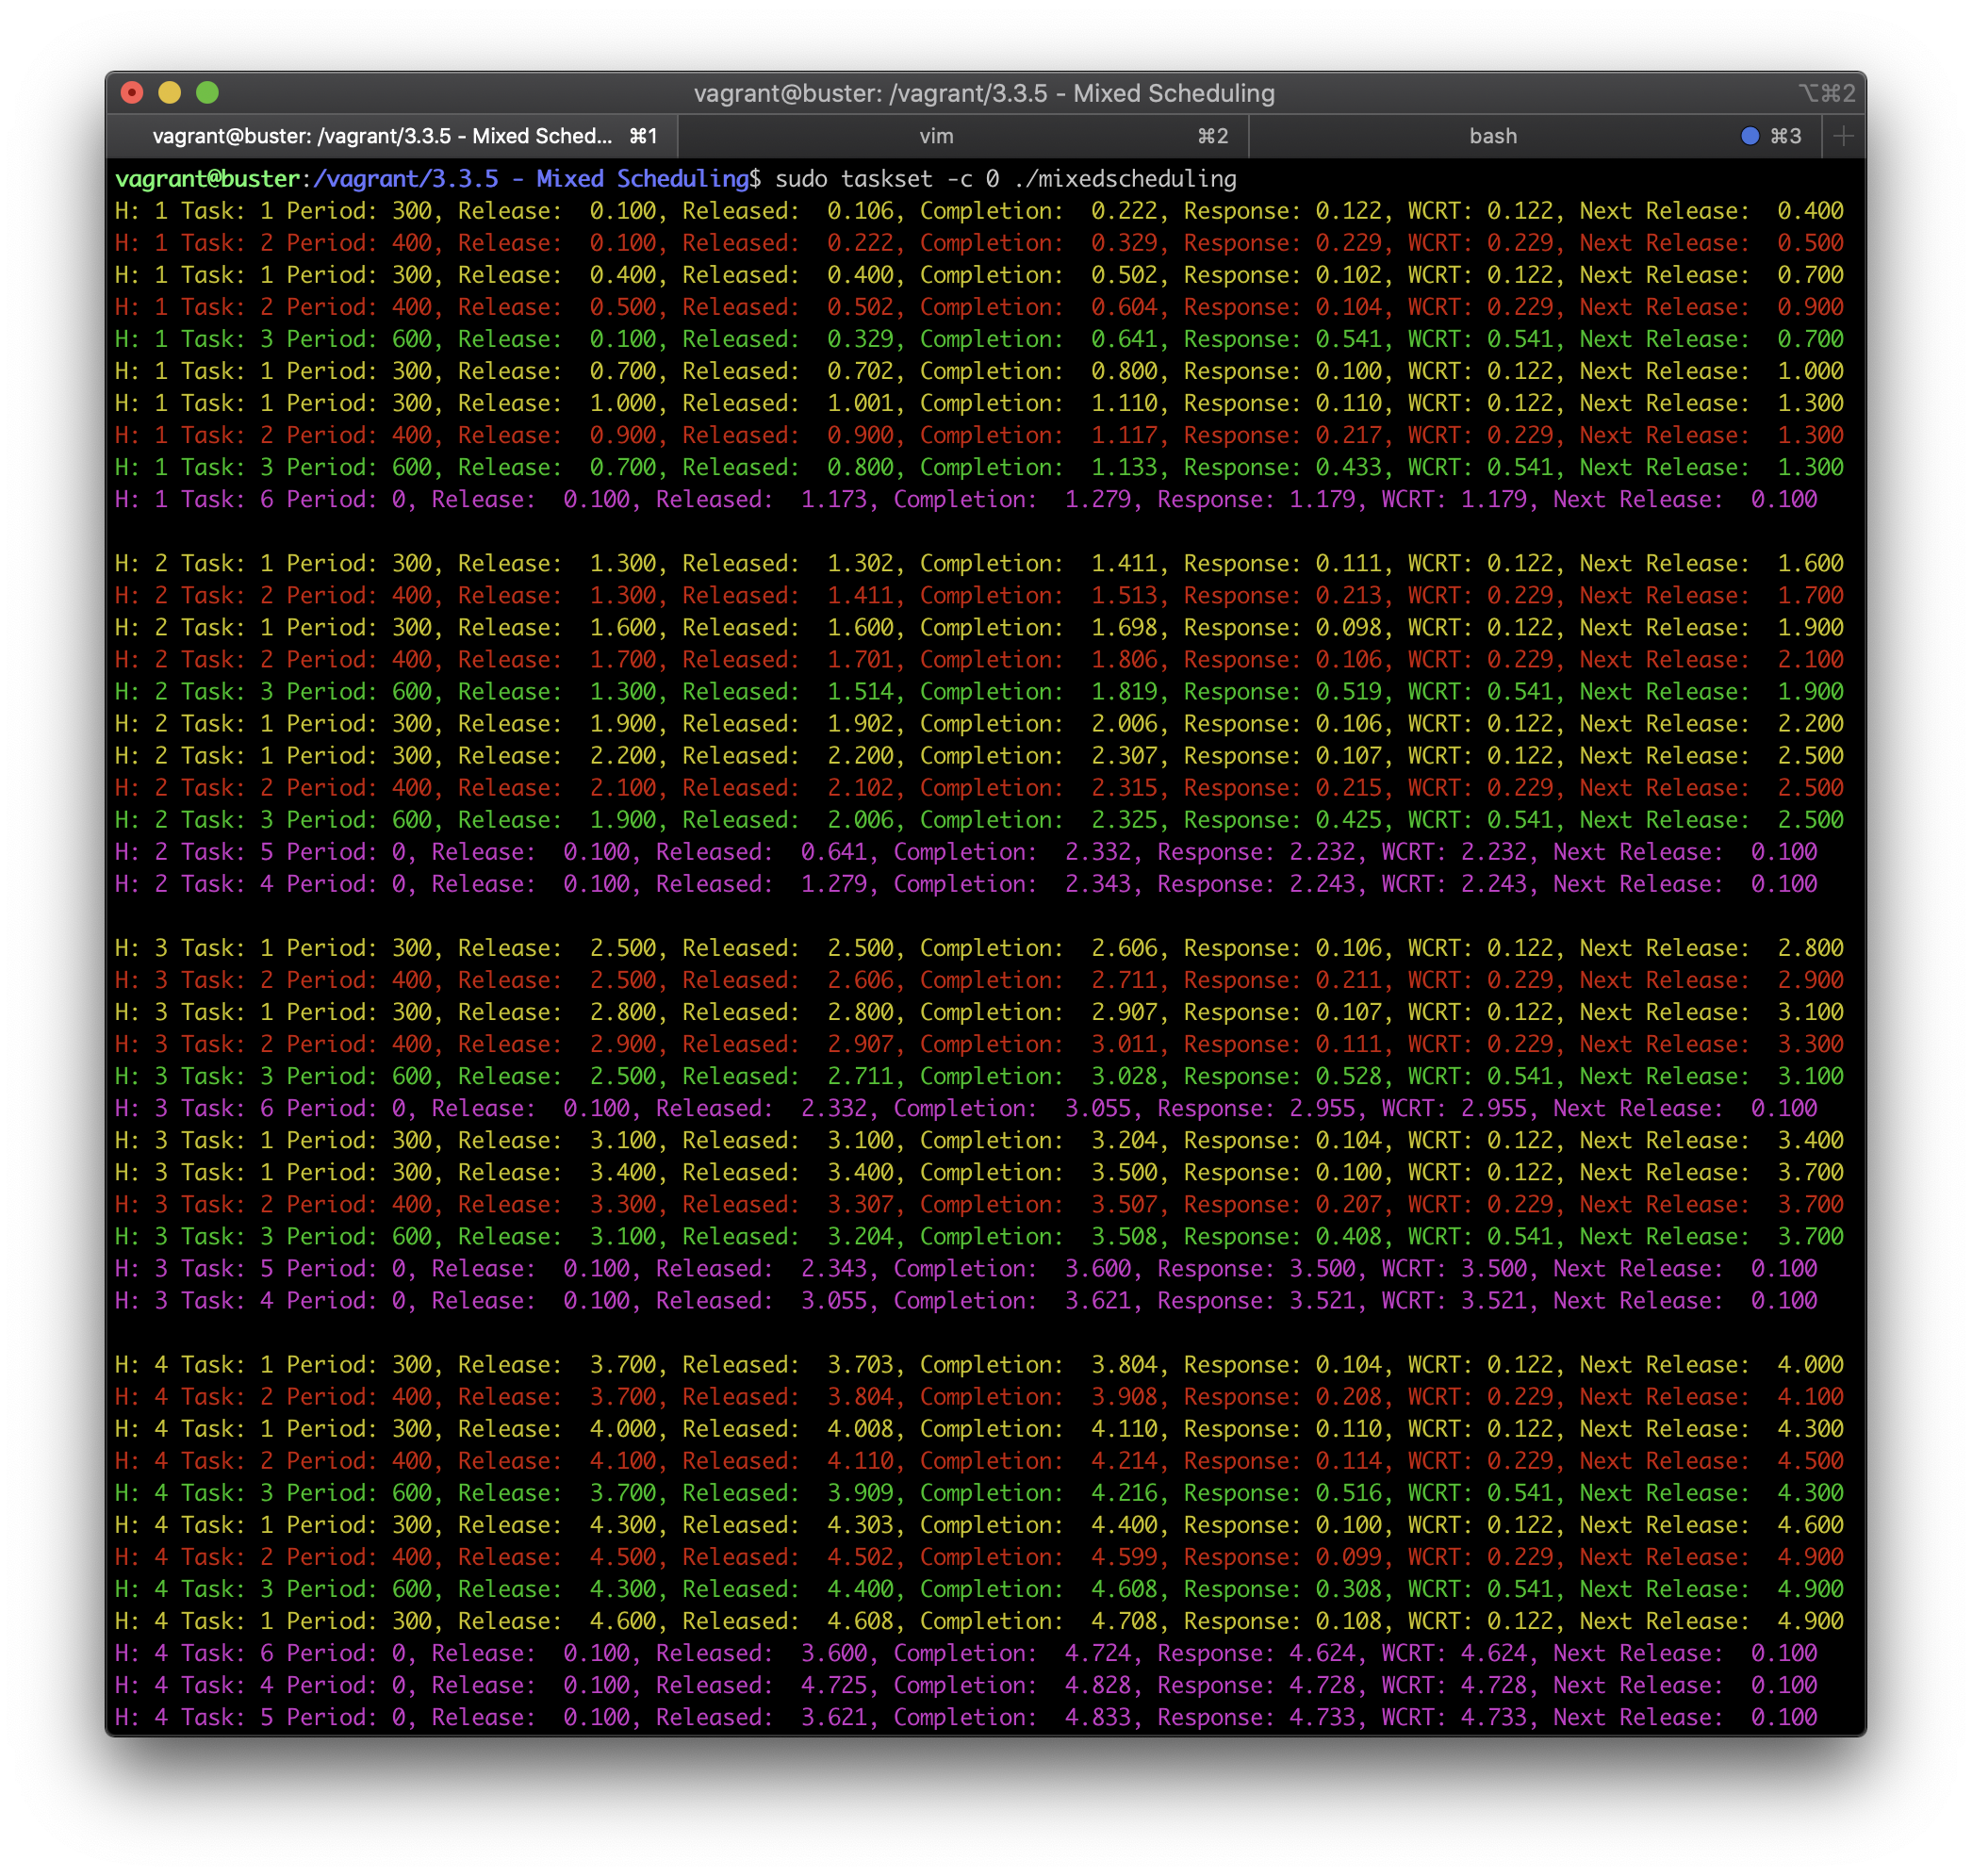
\includegraphics[width=\linewidth]{mixed-scheduling-output}
\end{figure}

From the output it can be seen that the program follows the same schedule as before, with the background tasks added. Since they have no timing requirements, they are started and completed sporadically, but manage to fill in the gaps left by the high priority tasks.

